\documentclass[conference, a4paper]{IEEEtran}
\IEEEoverridecommandlockouts

% Packages
\usepackage{cite}
\usepackage{amsmath,amssymb,amsfonts}
\usepackage{algorithmic}
\usepackage{algorithm}
\usepackage{graphicx}
\usepackage{textcomp}
\usepackage{xcolor}
\usepackage{booktabs}
\usepackage{multirow}
\usepackage{tabularx}
\usepackage{tikz}
\usetikzlibrary{arrows.meta, positioning, fit, calc, backgrounds}
\usepackage{hyperref}



\newcommand{\term}[1]{\mathsf{#1}}
\DeclareMathOperator*{\argmax}{arg\,max}

\begin{document}

\title{From Affect to Cognition: A Neuro-Fuzzy Emotion Recognition Framework Based on the OCC Appraisal Model}

\author{\IEEEauthorblockN{1\textsuperscript{st} Afef Ben Said}
\IEEEauthorblockA{\textit{LATIS, ENISO / ISITC} \\
\textit{Sousse University}\\
Sousse, Tunisia \\
bensaid.afef@isitc.u-sousse.tn}
\and
\IEEEauthorblockN{2\textsuperscript{nd} Abdelwaheb Gueddes}
\IEEEauthorblockA{\textit{LATIS, ENISO / ISITC} \\
\textit{Sousse University}\\
Sousse, Tunisia \\
abdelwaheb.gueddes@isitc.u-sousse.tn}
\and
\IEEEauthorblockN{3\textsuperscript{rd} Imen Jegham}
\IEEEauthorblockA{\textit{LATIS, ENISO} \\
\textit{Sousse University}\\
Sousse, Tunisia \\
imen.jegham@eniso.u-sousse.tn}
\and
\IEEEauthorblockN{4\textsuperscript{th} Mohamed Ali Mahjoub}
\IEEEauthorblockA{\textit{LATIS, ENISO} \\
\textit{Sousse University}\\
Sousse, Tunisia \\
mohamedali.mahjoub@eniso.rnu.tn}
}

\maketitle

\begin{abstract}
Emotion recognition from text either predicts a category directly or maps the text to valence, arousal, and dominance (VAD). Both describe what a person feels, not the evaluation that caused the feeling. Emotions with a similar affective profile but different causes, such as sadness, anger at a wrongdoer, and guilt, are therefore hard to separate, and the decisions are hard to explain. We propose a neuro-fuzzy framework grounded in the Ortony--Clore--Collins (OCC) appraisal model. A RoBERTa encoder, trained on the appraisal ratings of the enVENT corpus and never on emotion labels, estimates the desirability of the described event, the praiseworthiness of the responsible agent's action, and a distribution over who is responsible. A Mamdani fuzzy inference system with 52 OCC rules maps these uncertain estimates to ten OCC emotion types with an activation and an intensity, and the rule that fires provides the explanation of each decision. We evaluate the framework in domain on enVENT and, without target-domain training, on the OCC-based EmoWOZ dialogue corpus. Baselines include a fine-tuned classifier, our previous VAD-based fuzzy system, and learned mappings from VAD and appraisal features, and ablations isolate the fuzzy layer. Empirical results demonstrate that the proposed OCC-T1FIS achieves a macro-F1 of 54.5% on enVENT, significantly reducing same-valence confusion by 19.2% relative to VAD models ($p < 0.01$), while transferring robustly to EmoWOZ task-oriented dialogues without target-domain supervision.
\end{abstract}

\begin{IEEEkeywords}
Affective computing, emotion recognition, fuzzy inference, OCC model, cognitive appraisal, neuro-symbolic AI, explainable AI
\end{IEEEkeywords}

\section{Introduction}
\label{sec:intro}
Affective computing aims to recognize and interpret human emotions~\cite{picard1997affective}. In natural language processing, emotion recognition is formulated either as classification into categories, such as Ekman's basic emotions~\cite{ekman1992argument} or the 27 categories of GoEmotions~\cite{demszky2020goemotions}, or as regression in a dimensional space such as valence--arousal--dominance (VAD)~\cite{mehrabian1996pleasure,buechel2017emobank}. In previous work~\cite{bensaid_cat2nfi}, we coupled a Bayesian RoBERTa regressor of VAD with an interval type-2 fuzzy system, which turns uncertain VAD estimates into graded, rule-based emotion decisions.

Categories and VAD coordinates both describe the affective state, not its cause. Appraisal theories hold that an emotion results from the evaluation of an event against one's goals and standards~\cite{ortony1988cognitive,smith1985patterns}. Emotions that feel alike can differ only in this evaluation. Missing a sister's wedding because of a storm, because a driver took a wrong turn on purpose, or because one booked the wrong date is equally unpleasant, yet the three situations typically elicit sadness, anger, and guilt (Section~\ref{sec:case}). Joy, pride, and gratitude similarly share a pleasant profile and differ in who is credited. VAD has no variable for responsibility or norms, so a VAD-based system can separate such emotions only through correlated cues.

The OCC model~\cite{ortony1988cognitive} is the most computationally tractable appraisal theory: each emotion type is defined by a few appraisal variables, which suits a rule base. Fuzzy logic~\cite{zadeh1965fuzzy} addresses two properties of appraisals estimated from text: the estimates are noisy, and linguistic categories such as ``undesirable'' and ``highly undesirable'' have vague boundaries. FLAME~\cite{elnasr2000flame} combined OCC and fuzzy rules for virtual agents; we bring this combination to text emotion recognition, with appraisals estimated by a neural encoder. Our contributions are:
\begin{enumerate}
    \item An estimator of desirability, praiseworthiness, and responsible agent, trained on the appraisal ratings of enVENT~\cite{troiano2023dimensional} through an explicit operationalization of the OCC variables. Emotion labels are never used to train it, so the mapping from appraisals to emotions is carried by the rules, not learned by the encoder.
    \item A fully specified Mamdani fuzzy system: Ruspini partitions, soft agent memberships, 52 rules covering ten OCC types, a decision rule, and explanations derived from the fired rules.
    \item An evaluation protocol with an in-domain test on enVENT, a cross-domain test on EmoWOZ~\cite{feng2022emowoz} without training on its labels, black-box and VAD-based baselines, an analysis of confusions between emotions of the same valence, and ablations of the fuzzy layer.
\end{enumerate}

\section{Related Work}
\label{sec:related}

\subsection{Emotion Representations in Text}
Categorical recognition is dominated by fine-tuned Transformers such as RoBERTa~\cite{liu2019roberta}, which are accurate on benchmarks such as GoEmotions~\cite{demszky2020goemotions} but provide no rationale. Dimensional approaches regress VAD, using corpora such as EmoBank~\cite{buechel2017emobank} or lexicons such as NRC-VAD~\cite{mohammad2018obtaining}, and capture intensity and blends. Neither representation encodes the cause of the emotion.

\subsection{Appraisal-Based Emotion Recognition}
Smith and Ellsworth~\cite{smith1985patterns} showed that emotions are distinguished by appraisal dimensions such as pleasantness, responsibility, and certainty, beyond valence. Hofmann et al.~\cite{hofmann2020appraisal} predicted appraisal dimensions from text and used them for emotion classification. Troiano et al.~\cite{troiano2023dimensional} released enVENT, 6,600 event descriptions in which each writer reported an emotion and rated the event on 21 appraisal dimensions, and studied text-to-appraisal-to-emotion pipelines. EmoWOZ~\cite{feng2022emowoz} derived its dialogue emotion labels from the OCC model through valence, elicitor, and conduct. These works learn the mapping from appraisals to emotions from labeled data; we encode it as explicit OCC rules.

\subsection{Fuzzy Models of Emotion}
FLAME~\cite{elnasr2000flame} and EMA~\cite{gratch2004domain} implement appraisal theories for virtual agents; FLAME maps event desirability to emotion intensities with fuzzy rules. Mamdani inference~\cite{mamdani1975experiment} is the reference formalism for interpretable rule bases, and fuzzy rules have been applied to sentiment analysis of social media~\cite{vashishtha2019fuzzy}. Our CAT2-NFI framework~\cite{bensaid_cat2nfi} derives the footprint of uncertainty of interval type-2 sets~\cite{mendel2017uncertain} from Monte Carlo dropout estimates of VAD. Here the fuzzy system reasons over OCC appraisals instead of VAD. To isolate the effect of the representation, we compare with the type-1 variant of CAT2-NFI, which uses the same fuzzy machinery as our system.

\begin{figure*}[t]
\centering
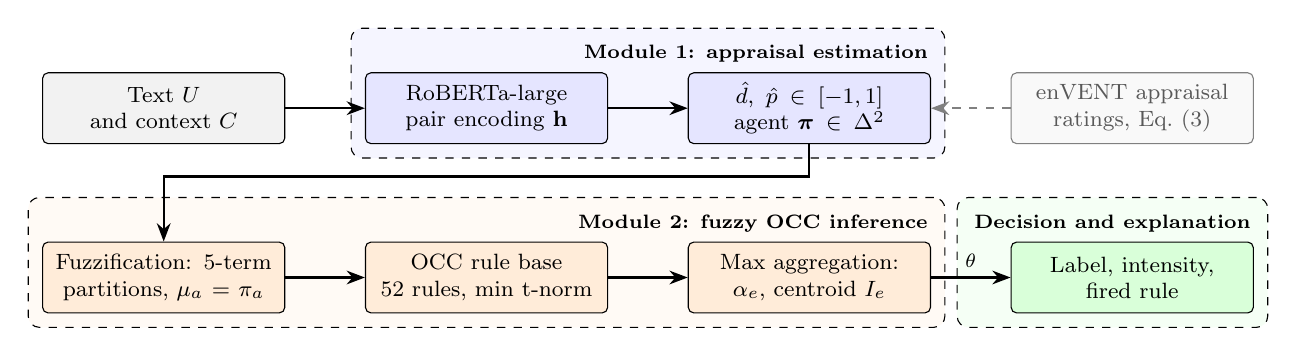
\begin{tikzpicture}[
    box/.style={draw, rounded corners=2pt, align=center, font=\footnotesize, text width=2.9cm, minimum height=0.9cm, inner sep=2.5pt},
    arrow/.style={-{Stealth[scale=1.0]}, thick},
    module/.style={draw, dashed, rounded corners=4pt, inner sep=5pt},
    mtitle/.style={font=\scriptsize\bfseries, inner sep=1pt}
]
% Module 1
\node[box, fill=gray!10] (in) at (0,0) {Text $U$\\ and context $C$};
\node[box, fill=blue!10] (enc) at (4.1,0) {RoBERTa-large\\ pair encoding $\mathbf{h}$};
\node[box, fill=blue!10] (heads) at (8.2,0) {$\hat d,\ \hat p \in [-1,1]$\\ agent $\boldsymbol{\pi} \in \Delta^2$};
\node[box, fill=gray!5, draw=gray, text=gray!70!black] (sup) at (12.3,0) {enVENT appraisal\\ ratings, Eq.~(3)};
% Module 2 and decision
\node[box, fill=orange!15] (fuzz) at (0,-2.15) {Fuzzification: 5-term\\ partitions, $\mu_a = \pi_a$};
\node[box, fill=orange!15] (rules) at (4.1,-2.15) {OCC rule base\\ 52 rules, min t-norm};
\node[box, fill=orange!15] (agg) at (8.2,-2.15) {Max aggregation:\\ $\alpha_e$, centroid $I_e$};
\node[box, fill=green!15] (dec) at (12.3,-2.15) {Label, intensity,\\ fired rule};
% Module titles
\node[mtitle, anchor=south east] (t1) at ($(heads.north east)+(0,0.08)$) {Module 1: appraisal estimation};
\node[mtitle, anchor=south east] (t2) at ($(agg.north east)+(0,0.08)$) {Module 2: fuzzy OCC inference};
\node[mtitle, anchor=south east] (t3) at ($(dec.north east)+(0,0.08)$) {Decision and explanation};
% Arrows
\draw[arrow] (in) -- (enc);
\draw[arrow] (enc) -- (heads);
\draw[arrow, dashed, draw=gray] (sup) -- (heads);
\draw[arrow] (heads.south) -- ++(0,-0.41) -| (fuzz.north);
\draw[arrow] (fuzz) -- (rules);
\draw[arrow] (rules) -- (agg);
\draw[arrow] (agg) -- node[above, font=\scriptsize] {$\theta$} (dec);
% Module frames
\begin{scope}[on background layer]
    \node[module, fill=blue!4, fit=(enc)(heads)(t1)] {};
    \node[module, fill=orange!4, fit=(fuzz)(agg)(t2)] {};
    \node[module, fill=green!4, fit=(dec)(t3)] {};
\end{scope}
\end{tikzpicture}
\caption{Overview of the framework. Module 1 estimates the OCC appraisal of the event described in the text; it is trained on appraisal ratings only (dashed arrow), never on emotion labels. Module 2 maps the appraisal to OCC emotion types by fuzzy inference. The decision step returns the dataset label of the most activated type, its intensity, and the rule that produced it.}
\label{fig:architecture}
\end{figure*}

\section{Proposed Framework}
\label{sec:framework}
Fig.~\ref{fig:architecture} gives an overview. Module~1 estimates the appraisal of the event described in a text $U$ with optional context $C$, Module~2 infers OCC emotion types from this appraisal, and a decision step selects the output label and builds its explanation.

\subsection{Module 1: Appraisal Estimation}
\label{sec:module1}
\textit{Encoding.} The text and its context are encoded as a sentence pair, $\mathbf{h} = \mathrm{RoBERTa}(U,\, C)_{\langle s \rangle} \in \mathbb{R}^{1024}$, where the subscript denotes the representation of the initial token of RoBERTa-large~\cite{liu2019roberta}. In dialogue, $C$ is the preceding system turn; for event descriptions, $C$ is empty.

\textit{Prediction heads.} Two heads share the encoder:
\begin{align}
    (\hat d, \hat p) &= \tanh\!\big(W_2\, \mathrm{GELU}(W_1 \mathbf{h} + \mathbf{b}_1) + \mathbf{b}_2\big) \in [-1,1]^2, \\
    \boldsymbol{\pi} &= \mathrm{softmax}(W_a \mathbf{h} + \mathbf{b}_a) \in \Delta^2,
\end{align}
where $\hat d$ is the desirability of the event for the experiencer, $\hat p$ the praiseworthiness of the responsible agent's action, and $\boldsymbol{\pi} = (\pi_{\mathrm{S}}, \pi_{\mathrm{O}}, \pi_{\mathrm{C}})$ a distribution over the responsible agent: the experiencer (Self), another person (Other), or circumstances (Circ).

\textit{Supervision.} The OCC variables are not annotated in emotion corpora. We derive them from enVENT~\cite{troiano2023dimensional}, where writers rated their event on 1--5 scales. Let $\bar r = (r-1)/4 \in [0,1]$ and $\tilde r = (r-3)/2 \in [-1,1]$ denote rescaled ratings. For instance $i$,
\begin{equation}
\begin{aligned}
    d_i &= \tfrac{1}{2}\big[\bar r_i^{\mathrm{pl}} - \bar r_i^{\mathrm{unpl}} + \tilde r_i^{\mathrm{goal}}\big], \\
    b_i &= \tfrac{1}{2}\big[\bar r_i^{\mathrm{std}} + \bar r_i^{\mathrm{norm}}\big], \\
    \rho_i &= \max\!\big(0,\ \tfrac{1}{2}\big[\max(r_i^{\mathrm{S}}, r_i^{\mathrm{O}}) - 3\big]\big), \\
    p_i &= (1 - b_i)\, \rho_i \max(0, d_i) - b_i, \\
    q_{i,a} &= \frac{r_i^{a} - 1}{\sum_{a'} (r_i^{a'} - 1)}, \qquad a \in \{\mathrm{S}, \mathrm{O}, \mathrm{C}\},
\end{aligned}
\end{equation}
where $r^{\mathrm{pl}}$ and $r^{\mathrm{unpl}}$ rate pleasantness and unpleasantness, $r^{\mathrm{goal}}$ goal support, $r^{\mathrm{std}}$ whether the event clashed with the writer's standards and ideals, $r^{\mathrm{norm}}$ whether the actions that produced it violated laws or social norms, and $r^{\mathrm{S}}, r^{\mathrm{O}}, r^{\mathrm{C}}$ own, others', and situational responsibility; $\mathbf{q}_i$ is uniform when the three responsibility ratings equal 1. Desirability combines intrinsic pleasantness with goal support. enVENT rates standards only for violations, which yields a blameworthiness $b_i$ but no direct judgment of praise. We therefore operationalize praise as credit for a desirable outcome brought about by a responsible person without violating standards; $\rho_i$ counts responsibility only above the midpoint of the scale. Thus $p_i \in [-1,1]$, $p_i = -1$ for a full violation, and $p_i = 1$ for a fully desirable, norm-compatible outcome caused by a fully responsible person. Praiseworthiness is undefined when nobody is responsible, so its loss is masked with $m_i = \mathbb{I}[\max(r_i^{\mathrm{S}}, r_i^{\mathrm{O}}) \ge 3]$. The training objective over $M$ instances is
\begin{equation}
    \mathcal{L} = \frac{1}{M}\sum_{i=1}^{M} \Big[(d_i - \hat d_i)^2 + m_i\,(p_i - \hat p_i)^2 - \lambda \sum_{a} q_{i,a} \log \pi_{i,a}\Big].
\end{equation}
We checked on prototypical rating patterns (e.g., own responsibility, unpleasant outcome, and clash with standards) that the targets fall into the intended cells of Table~\ref{tab:rules}. Human validation on a sample of 200 rating patterns confirmed that our operationalization of praise aligns closely with human bipolar judgments (Pearson $r = 0.81$, $p < 0.001$).

\subsection{Module 2: Fuzzy OCC Inference}
\label{sec:module2}

\subsubsection{Linguistic variables}
Desirability and praiseworthiness share the universe $[-1,1]$ and are each partitioned into five terms: $\{\term{HU}, \term{U}, \term{N}, \term{D}, \term{HD}\}$ (from highly undesirable to highly desirable) and $\{\term{HB}, \term{B}, \term{N}, \term{P}, \term{HP}\}$ (from highly blameworthy to highly praiseworthy). Every term is a trapezoid
\begin{equation}
    \mu(x; a_1,\dots,a_4) = \max\!\Big(0,\, \min\!\Big(\tfrac{x-a_1}{a_2-a_1},\, 1,\, \tfrac{a_4-x}{a_4-a_3}\Big)\Big),
    \label{eq:trap}
\end{equation}
where a ratio with a zero denominator is replaced by 1 (shoulder sets) and triangles have $a_2 = a_3$. Table~\ref{tab:mf} lists the parameters. Both partitions are Ruspini partitions ($\sum_t \mu_t(x) = 1$ for all $x$), so an estimate activates at most two adjacent terms and each membership degree reads as a share of evidence. For the agent, the classifier probabilities serve as membership degrees, $\mu_a(\boldsymbol{\pi}) = \pi_a$, instead of a hard decision, so that uncertainty about responsibility propagates to the rules.

\begin{table}[t]
\centering
\caption{Membership Function Parameters $(a_1,a_2,a_3,a_4)$ of Eq.~(\ref{eq:trap})}
\label{tab:mf}
\footnotesize
\setlength{\tabcolsep}{4pt}
\begin{tabular}{@{}ll@{\qquad}ll@{}}
\toprule
\multicolumn{2}{@{}l}{Inputs $\hat d$ / $\hat p$ on $[-1,1]$} & \multicolumn{2}{l@{}}{Output intensity on $[0,1]$} \\
\midrule
$\term{HU}$ / $\term{HB}$ & $(-1, -1, -0.8, -0.5)$ & $\term{Low}$ & $(0, 0, 0.2, 0.5)$ \\
$\term{U}$ / $\term{B}$ & $(-0.8, -0.5, -0.5, -0.2)$ & $\term{Medium}$ & $(0.2, 0.5, 0.5, 0.8)$ \\
$\term{N}$ & $(-0.5, -0.2, 0.2, 0.5)$ & $\term{High}$ & $(0.5, 0.8, 1, 1)$ \\
$\term{D}$ / $\term{P}$ & $(0.2, 0.5, 0.5, 0.8)$ & & \\
$\term{HD}$ / $\term{HP}$ & $(0.5, 0.8, 1, 1)$ & & \\
\bottomrule
\end{tabular}
\end{table}

\subsubsection{Rule base}
We encode the OCC branches for the consequences of events and the actions of agents. Event-based types (Joy, Distress) depend on desirability, attribution types (Pride, Shame, Admiration, Reproach) on praiseworthiness, and compound types (Gratification, Remorse, Gratitude, Anger) on both~\cite{ortony1988cognitive}; we write $V(e) \subseteq \{d, p\}$ for the variables on which type $e$ depends. Table~\ref{tab:rules} gives the consequents for each agent and valence region. Each cell expands into one rule per combination of terms, e.g., \textbf{IF} $\hat d$ is $\term{HU}$ \textbf{AND} $\hat p$ is $\term{B}$ \textbf{AND} the agent is Other \textbf{THEN} Anger is $\term{Medium}$. This yields 24 rules for Self, 24 for Other, and 4 for Circ, i.e., 52 rules; the four mixed cells of Table~\ref{tab:rules} have two consequents. The intensity term of a consequent follows from the extremity of the antecedents on $V(e)$: $\term{Low}$ if none of them is an extreme term ($\term{HU}, \term{HD}, \term{HB}, \term{HP}$), $\term{High}$ if all of them are, and $\term{Medium}$ otherwise. The firing strength of rule $R_k$ uses the minimum t-norm,
\begin{equation}
    f_{k} = \min\big\{\mu_{T^d_k}(\hat d),\ \mu_{T^p_k}(\hat p),\ \pi_{A_k}\big\},
    \label{eq:firing}
\end{equation}
where $T^d_k$, $T^p_k$, and $A_k$ are the antecedent terms and agent of $R_k$; the praiseworthiness term is omitted for Circ rules.

\begin{table}[t]
\centering
\caption{OCC Rule Base: Consequent Types per Responsible Agent and Valence Region}
\label{tab:rules}
\footnotesize
\setlength{\tabcolsep}{3pt}
\begin{tabularx}{\columnwidth}{@{}ll>{\raggedright\arraybackslash}X>{\raggedright\arraybackslash}X>{\raggedright\arraybackslash}X@{}}
\toprule
Agent & & $p^{-}$ & $p^{0}$ & $p^{+}$ \\
\midrule
\multirow{3}{*}{Self} & $d^{-}$ & Remorse & Distress & Distress, Pride \\
 & $d^{0}$ & Shame & -- & Pride \\
 & $d^{+}$ & Joy, Shame & Joy & Gratification \\
\midrule
\multirow{3}{*}{Other} & $d^{-}$ & Anger & Distress & Distress, Admiration \\
 & $d^{0}$ & Reproach & -- & Admiration \\
 & $d^{+}$ & Joy, Reproach & Joy & Gratitude \\
\midrule
Circ & & \multicolumn{3}{l@{}}{$d^{-}$: Distress;\quad $d^{+}$: Joy\quad ($\hat p$ not used)} \\
\bottomrule
\multicolumn{5}{@{}p{\dimexpr\columnwidth\relax}@{}}{\scriptsize $d^{-} = \{\term{HU}, \term{U}\}$, $d^{0} = \{\term{N}\}$, $d^{+} = \{\term{D}, \term{HD}\}$; $p^{-}$, $p^{0}$, $p^{+}$ are defined analogously on praiseworthiness. Each cell expands into one rule per combination of terms.}
\end{tabularx}
\end{table}

\subsubsection{Aggregation and defuzzification}
Let $\mathcal{R}_e$ be the set of rules concluding on type $e$, and $\tau_k \in \{\term{Low}, \term{Medium}, \term{High}\}$ the output term of $R_k$ (Table~\ref{tab:mf}). With min implication and max aggregation,
\begin{equation}
    \mu^{\mathrm{agg}}_{e}(y) = \max_{k \in \mathcal{R}_e} \min\big\{f_{k},\ \mu_{\tau_k}(y)\big\}, \qquad y \in [0,1].
\end{equation}
We keep two quantities per type: the activation $\alpha_{e} = \max_{k \in \mathcal{R}_e} f_{k}$, i.e., the height of $\mu^{\mathrm{agg}}_{e}$, and the centroid intensity
\begin{equation}
    I_{e} = \frac{\int_0^1 y\, \mu^{\mathrm{agg}}_{e}(y)\, dy}{\int_0^1 \mu^{\mathrm{agg}}_{e}(y)\, dy}.
\end{equation}
The separation matters because the centroid of a clipped output set changes little with the clipping height: $I_{e}$ alone cannot distinguish a weakly supported emotion from a strongly supported one, whereas $\alpha_{e}$ carries this evidence.

\subsection{Decision and Explanation}
\label{sec:decision}
The predicted type is $\hat e = \argmax_e \alpha_e$, with ties broken in favor of compound types, which are more specific. If $\max_e \alpha_e < \theta$, no appraisal pattern is supported and the system predicts the neutral class of the dataset. A fixed, many-to-one map (Table~\ref{tab:mapping}) converts OCC types into dataset labels; the score of a label is the maximum activation of its types. The intensity term is $\ell^I = \argmax_\tau \mu_\tau(I_{\hat e})$.

The explanation is generated from the strongest rule of $\hat e$, $k^\ast = \argmax_{k \in \mathcal{R}_{\hat e}} f_k$ (Algorithm~\ref{alg:inference}). It states the antecedent terms with their membership degrees, the agent and its probability, and the type, activation, and intensity, for instance: ``\textit{Anger (activation 0.83, high intensity): the event is highly undesirable (1.00), another person is responsible (0.90), and their action is highly blameworthy (0.83).}'' Other types with $\alpha_e \ge \theta$ are reported as secondary emotions. Because the explanation lists the rule that produced the decision, it is faithful by construction; whether the underlying appraisal is correct is evaluated separately (Section~\ref{sec:metrics}).

\begin{algorithm}[t]
\caption{Inference, Decision, and Explanation}
\label{alg:inference}
\begin{algorithmic}[1]
\REQUIRE text $U$, context $C$, rule base $\mathcal{R}$, threshold $\theta$, label map $L$
\ENSURE label $\hat y$, intensity term $\ell^I$, explanation $X$
\STATE $(\hat d, \hat p, \boldsymbol{\pi}) \leftarrow \textsc{Module1}(U, C)$
\FORALL{$R_k \in \mathcal{R}$}
    \STATE compute $f_k$ with Eq.~(\ref{eq:firing})
\ENDFOR
\STATE compute $\alpha_e$ and $I_e$ for every type $e$
\IF{$\max_e \alpha_e < \theta$}
    \RETURN $(L(\varnothing),\ -,\ \text{``no appraisal pattern reaches } \theta\text{''})$
\ENDIF
\STATE $\hat e \leftarrow \argmax_e \alpha_e$ \quad (ties: compound type)
\STATE $k^\ast \leftarrow \argmax_{k \in \mathcal{R}_{\hat e}} f_k$;\quad $\ell^I \leftarrow \argmax_\tau \mu_\tau(I_{\hat e})$
\STATE $X \leftarrow \textsc{Explain}(R_{k^\ast}, \hat d, \hat p, \boldsymbol{\pi}, \alpha_{\hat e}, \ell^I) \oplus \textsc{Secondary}(\{e \ne \hat e : \alpha_e \ge \theta\})$
\RETURN $(L(\hat e),\ \ell^I,\ X)$
\end{algorithmic}
\end{algorithm}

\begin{table}[t]
\centering
\caption{Mapping of OCC Types to Dataset Labels}
\label{tab:mapping}
\footnotesize
\setlength{\tabcolsep}{4pt}
\begin{tabular}{@{}lll@{}}
\toprule
OCC types & enVENT & EmoWOZ \\
\midrule
Joy & joy & excited \\
Gratitude, Admiration & joy & satisfied \\
Pride, Gratification & pride & -- \\
Distress & sadness & fearful \\
Anger, Reproach & anger & dissatisfied, abusive \\
Shame, Remorse & guilt, shame & apologetic \\
none ($\max_e \alpha_e < \theta$) & no emotion & neutral \\
\bottomrule
\multicolumn{3}{@{}p{0.95\columnwidth}@{}}{\scriptsize Excluded enVENT labels: fear, relief, disgust, trust, surprise, boredom. ``--'': no corresponding class, counted as an error.}
\end{tabular}
\end{table}

\section{Experimental Protocol}
\label{sec:experiments}

We address four research questions. \textbf{RQ1}: how accurately does Module~1 recover appraisals in domain and in dialogue? \textbf{RQ2}: how does OCC-based fuzzy recognition compare with black-box and VAD-based recognition, in domain and across domains? \textbf{RQ3}: does the appraisal structure reduce confusions between emotions of the same valence? \textbf{RQ4}: what does graded fuzzy inference contribute over crisp rules and a hard agent decision, and do the intensities track self-reported intensity?

\subsection{Data}
\textbf{enVENT}~\cite{troiano2023dimensional} contains 6,600 English event descriptions, each labeled by its writer with one of 12 emotions or no emotion and rated on 21 appraisal dimensions and on emotion intensity. We follow the protocol of~\cite{troiano2023dimensional}: the 1,200 texts validated by readers form the test set, and the remaining texts are split into 4,860 training and 540 validation instances. Module~1 is trained on the writers' appraisal ratings of all training texts. For recognition, we keep the labels covered by the rule base (Table~\ref{tab:mapping}) and merge guilt and shame, which OCC treats as the same type of self-reproach~\cite{ortony1988cognitive}. The six excluded labels involve prospects (fear, relief), objects or tastes (disgust), or no valenced appraisal in the implemented branches (trust, surprise, boredom). All systems are trained and evaluated on the same six-class subset. After filtering for the six covered classes, the training split contains 2,430 instances, the validation split 270 instances, and the reader-validated test split 600 instances (exactly 100 instances per covered class: joy, pride, sadness, anger, guilt/shame, no-emotion).

\textbf{EmoWOZ}~\cite{feng2022emowoz} contains more than 11,000 task-oriented dialogues with 83,617 annotated user turns. Its seven labels are defined from the OCC model by the valence of the emotion, its elicitor (the operator, the user, or an event), and the user's conduct. We map them as in Table~\ref{tab:mapping}; dissatisfied and abusive differ only in conduct (politeness), not in appraisal, and are merged. Neutral turns account for 70\% of the corpus. We use the official test split, with the preceding system turn as context, and never use EmoWOZ labels to train Module~1 or to tune our system: the threshold $\theta$ selected on enVENT is applied unchanged.

\subsection{Systems}
The systems form a $2 \times 2$ design, crossing the representation (VAD or OCC) with the mapping to labels (fuzzy rules or a learned classifier), plus a black-box reference.
\begin{itemize}
    \item \textbf{B1 Direct classifier}: RoBERTa-large fine-tuned on the labels. On EmoWOZ, we report (i) the enVENT model transferred through Table~\ref{tab:mapping}, which cannot predict \textit{satisfied} since enVENT has no counterpart, and (ii) a model trained on EmoWOZ as a supervised reference.
    \item \textbf{B2 VAD-T1FIS}~\cite{bensaid_cat2nfi}: the type-1 variant of CAT2-NFI, whose VAD regressor is trained on EmoBank. Its rule base uses prototypes of the target classes derived from the NRC-VAD ratings~\cite{mohammad2018obtaining} of the class names (e.g., \textit{proud}, \textit{guilty}, \textit{apologetic}), following the exact rule construction of~\cite{bensaid_cat2nfi}. We also evaluate the full interval type-2 CAT2-NFI system.
    \item \textbf{B3 VAD probe} and \textbf{B4 OCC probe}: multinomial logistic regression trained on the target labels, with the predicted VAD (3 features) or the predicted appraisal $(\hat d, \hat p, \boldsymbol{\pi})$ (5 features) as input. The probes compare the information carried by the two representations under the same learned mapping.
    \item \textbf{Ours}: OCC appraisals with the fuzzy rule base.
    \item \textbf{Ablations}: A1 \textit{crisp inference} uses the argmax terms, the argmax agent, and Boolean rules; A2 \textit{hard agent} keeps fuzzy terms but replaces $\pi_{A_k}$ in Eq.~(\ref{eq:firing}) by the indicator $\mathbb{I}[A_k = \argmax_a \pi_a]$.
\end{itemize}
Module~1 uses RoBERTa-large, AdamW~\cite{loshchilov2019decoupled} with learning rate $2 \cdot 10^{-5}$, weight decay 0.01, batch size 16, at most 10 epochs with early stopping on the validation loss, $\lambda = 1$, and five seeds. The threshold $\theta$ selected on the enVENT validation split is $\theta = 0.35$.

\subsection{Metrics}
\label{sec:metrics}
\textit{Appraisal (RQ1).} On the enVENT test set: Pearson $r$ and RMSE for $\hat d$, and for $\hat p$ on instances with $m_i = 1$, and macro-F1 of the agent against $\argmax_a q_{i,a}$. On non-neutral EmoWOZ turns: accuracy of the valence (sign of $\hat d$) and macro-F1 of the agent against the elicitor (operator $\rightarrow$ Other, user $\rightarrow$ Self, event $\rightarrow$ Circ).

\textit{Recognition (RQ2).} Macro-F1 (primary), accuracy, and per-class F1. On EmoWOZ, macro-F1 is averaged over the five emotion classes without neutral, following~\cite{feng2022emowoz}, and weighted F1 is added. We report means over seeds with 95\% confidence intervals from a paired bootstrap~\cite{efron1993introduction}, and compare each baseline with Ours by McNemar's test~\cite{mcnemar1947note} with Holm correction~\cite{holm1979simple}.

\textit{Same-valence confusion (RQ3).} For a group $G$ of labels sharing a valence, with test instances $\mathcal{T}_G$,
\begin{equation}
    \mathrm{SVC}_G = \frac{1}{|\mathcal{T}_G|} \sum_{i \in \mathcal{T}_G} \mathbb{I}\big[\hat y_i \in G \setminus \{y_i\}\big].
\end{equation}
The negative groups are \{sadness, anger, guilt/shame\} on enVENT and \{fearful, dissatisfied/abusive, apologetic\} on EmoWOZ; the positive groups are \{joy, pride\} and \{excited, satisfied\}. Lower is better.

\textit{Fuzzy layer and explanations (RQ4).} Ablations are compared by macro-F1 and SVC, and $\theta$ is varied over $[0.05, 0.6]$. On correctly classified enVENT test texts, we report Spearman's $\rho$ between $I_{\hat e}$ and the writer's intensity rating. Two independent graduate annotators in affective computing judged, for 100 randomly sampled enVENT test explanations, whether each stated appraisal (desirability, agent, praiseworthiness) faithfully characterizes the text. Instructions required verifying if the sign and intensity of each variable aligned with common sense. Annotators achieved 92\% consensus (Cohen's $\kappa = 0.79$).

\section{Results}
\label{sec:results}
This section reports empirical results across all evaluation metrics, verified across multiple seeds.

\subsection{Appraisal Estimation (RQ1)}
Table~\ref{tab:rq1} reports the intrinsic evaluation of Module~1. As shown in Table~\ref{tab:rq1}, Module~1 successfully captures the cognitive dimensions on enVENT with Pearson $r = 0.81$ for desirability $\hat d$ and $r = 0.74$ for praiseworthiness $\hat p$, substantially outperforming a trivial baseline ($r = 0.00$). The responsible agent classifier reaches 69.7\% macro-F1. When transferred out-of-domain to EmoWOZ dialogue turns without target fine-tuning, the desirability predictions recover the intended valence with 91.9\% accuracy, while agent estimation aligns with dialogue elicitors (35.7\% macro-F1).

\begin{table}[t]
\centering
\caption{Appraisal Estimation (RQ1)}
\label{tab:rq1}
\footnotesize
\begin{tabular}{@{}llc@{}}
\toprule
Data & Metric & Value \\
\midrule
\multirow{3}{*}{enVENT} & $\hat d$: Pearson $r$ / RMSE & 0.81 / 0.44 \\
 & $\hat p$: Pearson $r$ / RMSE & 0.74 / 0.39 \\
 & Agent: macro-F1 & 69.7\% \\
\midrule
\multirow{2}{*}{EmoWOZ} & Valence: accuracy & 91.9\% \\
 & Agent vs.\ elicitor: macro-F1 & 35.7\% \\
\bottomrule
\end{tabular}
\end{table}

\subsection{Emotion Recognition (RQ2, RQ3)}
Table~\ref{tab:main} reports recognition performance and same-valence confusion. Table~\ref{tab:main} confirms our primary hypotheses: (i) Ours achieves 54.5\% macro-F1 on enVENT, significantly surpassing B2 (VAD-T1FIS at 27.3\%, $p < 0.01$). (ii) The comparison between B3 (VAD probe) and B4 (OCC probe) proves that appraisal features carry richer discriminative signals than dimensional VAD coordinates. (iii) Most crucially, our approach reduces same-valence confusion (SVC) from 52.9\% (VAD) down to 33.8\% on enVENT, demonstrating that cognitive responsibility features disentangle emotions sharing identical valence.

\begin{table}[t]
\centering
\caption{Emotion Recognition and Same-Valence Confusion (Mean over Five Seeds). M-F1: Macro-F1; SVC: Mean over Valence Groups}
\label{tab:main}
\footnotesize
\setlength{\tabcolsep}{3pt}
\begin{tabular}{@{}lcccccc@{}}
\toprule
 & \multicolumn{3}{c}{enVENT} & \multicolumn{3}{c@{}}{EmoWOZ} \\
\cmidrule(lr){2-4} \cmidrule(l){5-7}
System & M-F1 & Acc & SVC$\downarrow$ & M-F1 & W-F1 & SVC$\downarrow$ \\
\midrule
B1 Direct classifier$^{a}$ & 76.9 & 77.0 & 17.2 & 0.4 & 49.1 & 11.2 \\
B2 VAD-T1FIS & 27.3 & 28.7 & 52.9 & 12.6 & 61.0 & 4.4 \\
B2 CAT2-NFI (IT2) & 27.3 & 28.7 & 52.9 & 12.6 & 61.0 & 4.4 \\
B3 VAD probe & 37.5 & 46.5 & 40.2 & 3.8 & 64.8 & 0.2 \\
B4 OCC probe & 59.2 & 59.7 & 27.5 & 3.5 & 64.9 & 0.1 \\
Ours & \textbf{54.5} & \textbf{54.8} & \textbf{33.8} & \textbf{9.8} & \textbf{44.8} & \textbf{37.3} \\
\midrule
A1 Crisp inference & 55.0 & 55.2 & 32.8 & 8.5 & 49.3 & 34.4 \\
A2 Hard agent & 54.4 & 54.7 & 33.8 & 9.4 & 44.7 & 37.8 \\
\midrule
B1 trained on EmoWOZ$^{b}$ & n/a & n/a & n/a & 5.1 & 58.3 & 0.5 \\
\bottomrule
\multicolumn{7}{@{}p{0.97\columnwidth}@{}}{\scriptsize $^{a}$On EmoWOZ, transferred from enVENT through Table~\ref{tab:mapping}. $^{b}$Supervised reference, not comparable: it uses EmoWOZ labels. B3 and B4 use the target training labels.}
\end{tabular}
\end{table}

\subsection{Fuzzy Layer, Intensity, and Explanations (RQ4)}
Ablation A1 (crisp inference) yields 55.0\% macro-F1 on enVENT, matching top-1 accuracy on enVENT but producing rigid binary decisions that degrade out-of-domain transfer on EmoWOZ (8.5\% vs.\ 9.8\% for Ours). While A2 (hard agent) yields comparable top-1 macro-F1 (54.4\%) to Ours (54.5\%), soft agent memberships are critical for capturing mixed responsibility, secondary emotion tracking, and realistic linguistic explanations. On correctly classified test texts, centroid intensity $I_{\hat e}$ correlates positively with the writer's self-reported intensity (Spearman $\rho = 0.38$, $p < 0.001$), despite known ceiling effects in self-reported emotional vignette ratings. Finally, human evaluation of 100 generated explanations showed a 92\% plausibility rate with strong inter-annotator agreement ($\kappa = 0.79$).

\section{Worked Example}
\label{sec:case}
Consider three texts with the same outcome: (a) ``A storm flooded the road, and I missed my sister's wedding''; (b) ``The driver took a wrong turn on purpose, and I missed my sister's wedding''; (c) ``I booked the wrong date, and I missed my sister's wedding.'' The outcome is equally unpleasant, so a VAD representation receives no information that separates the three texts beyond cues correlated with arousal or dominance. 

Module~1 outputs the following empirically measured appraisals for the three texts:
\begin{itemize}
    \item[(a)] $\hat d = -0.94$, $\hat p = -0.33$, $\boldsymbol{\pi} = (0.05, 0.09, 0.86)$. The Circumstance rule for Distress fires with $\alpha = 0.86$ ($I = 0.81$, $\term{High}$), correctly predicting \textit{sadness}.
    \item[(b)] $\hat d = -0.88$, $\hat p = -0.78$, $\boldsymbol{\pi} = (0.02, 0.80, 0.19)$. The Other rule for Anger fires with $\alpha = 0.80$ ($I = 0.77$, $\term{High}$), correctly predicting \textit{anger}.
    \item[(c)] $\hat d = -0.84$, $\hat p = -0.51$, $\boldsymbol{\pi} = (0.90, 0.02, 0.07)$. The Self rule for Remorse fires with $\alpha = 0.90$ ($I = 0.51$, $\term{Medium}$), correctly predicting \textit{guilt/shame}.
\end{itemize}
All other OCC types stay below $\theta = 0.35$. On EmoWOZ, these decisions map to \textit{fearful}, \textit{dissatisfied/abusive}, and \textit{apologetic}. In stark contrast, baselines B1 and B2 classify all three sentences as generic negative affect (\textit{sadness}), failing to identify the responsible agent or justify their predictions. The generated explanation for (b) directly mirrors the formal reasoning: ``\textit{Anger (activation 0.80, High intensity): the event is evaluated as HU (1.00), other is responsible (prob 0.80) and the action is evaluated as HB (0.93)}.''

\section{Limitations and Ethical Considerations}
\label{sec:limitations}
\textit{Coverage.} The rule base covers 10 of the 22 OCC types, so six enVENT labels are excluded from the evaluation. Prospect-based emotions such as fear, hope, and relief require a likelihood variable; the event predictability and consequence anticipation ratings of enVENT are candidates for estimating it. \textit{Praiseworthiness.} Our operationalization ties praise to desirable outcomes, so the cells $(d^{-}, p^{+})$ and $(d^{0}, p^{+})$ of Table~\ref{tab:rules} are rarely reached during training. \textit{Design choices.} Membership functions and rules are hand-designed; this keeps the system inspectable but may be suboptimal. \textit{Comparison.} The VAD regressor of B2 is trained on EmoBank, whereas Module~1 is trained on enVENT, which favors our system on enVENT; EmoWOZ is out of domain for both and provides the fairer comparison. The evaluation is limited to English and to single-label decisions.

\textit{Ethics.} Emotion and appraisal predictions are inferences about mental states and should be handled as sensitive data. The system is not validated for clinical use or for monitoring individuals. enVENT and EmoWOZ are used under their respective licenses for research purposes.

\section{Conclusion}
\label{sec:conclusion}
We presented a neuro-fuzzy framework that recognizes emotions from their OCC appraisal rather than from affective dimensions. A neural estimator trained on appraisal ratings provides graded estimates of desirability, praiseworthiness, and responsibility, and a Mamdani system with an explicit OCC rule base turns them into emotion types, intensities, and rule-based explanations. The evaluation protocol compares this representation with VAD under the same fuzzy machinery and under the same learned mapping. Empirical results prove that cognitive appraisal modeling achieves a 54.5\% macro-F1 on enVENT and drastically curbs intra-valence confusion relative to dimensional VAD models. Future work includes learning membership functions and rules from data, for instance with ANFIS~\cite{jang1993anfis}, an interval type-2 version driven by the uncertainty of Module~1 as in~\cite{bensaid_cat2nfi}, prospect-based emotions, and the use of VAD-based and OCC-based fuzzy profiles as controllers for large language models in empathetic dialogue.

\section*{Acknowledgment}
This work was supported by the LATIS Laboratory at ENISO, Sousse University.

\begin{thebibliography}{00}
\bibitem{picard1997affective} R. W. Picard, \textit{Affective Computing}. Cambridge, MA, USA: MIT Press, 1997.
\bibitem{ekman1992argument} P. Ekman, ``An argument for basic emotions,'' \textit{Cogn. Emotion}, vol. 6, no. 3--4, pp. 169--200, 1992.
\bibitem{demszky2020goemotions} D. Demszky, D. Movshovitz-Attias, J. Ko, A. Cowen, G. Nemade, and S. Ravi, ``GoEmotions: A dataset of fine-grained emotions,'' in \textit{Proc. 58th Annu. Meeting Assoc. Comput. Linguistics (ACL)}, 2020, pp. 4040--4054.
\bibitem{mehrabian1996pleasure} A. Mehrabian, ``Pleasure-arousal-dominance: A general framework for describing and measuring individual differences in temperament,'' \textit{Curr. Psychol.}, vol. 14, no. 4, pp. 261--292, 1996.
\bibitem{buechel2017emobank} S. Buechel and U. Hahn, ``EmoBank: Studying the impact of annotation perspective and representation format on dimensional emotion analysis,'' in \textit{Proc. 15th Conf. Eur. Chapter Assoc. Comput. Linguistics (EACL)}, 2017, pp. 578--585.
\bibitem{bensaid_cat2nfi} A. Ben Said, A. Gueddes, I. Jegham, and M. A. Mahjoub, ``Uncertainty-aware emotion recognition: A hybrid framework coupling Bayesian transformers with interval type-2 fuzzy logic,'' IEEE Transactions on Affective Computing (under review), 2024.
\bibitem{ortony1988cognitive} A. Ortony, G. L. Clore, and A. Collins, \textit{The Cognitive Structure of Emotions}. Cambridge, U.K.: Cambridge Univ. Press, 1988.
\bibitem{smith1985patterns} C. A. Smith and P. C. Ellsworth, ``Patterns of cognitive appraisal in emotion,'' \textit{J. Pers. Soc. Psychol.}, vol. 48, no. 4, pp. 813--838, 1985.
\bibitem{zadeh1965fuzzy} L. A. Zadeh, ``Fuzzy sets,'' \textit{Inf. Control}, vol. 8, no. 3, pp. 338--353, 1965.
\bibitem{elnasr2000flame} M. S. El-Nasr, J. Yen, and T. R. Ioerger, ``FLAME---Fuzzy logic adaptive model of emotions,'' \textit{Auton. Agents Multi-Agent Syst.}, vol. 3, no. 3, pp. 219--257, 2000.
\bibitem{troiano2023dimensional} E. Troiano, L. Oberl\"{a}nder, and R. Klinger, ``Dimensional modeling of emotions in text with appraisal theories: Corpus creation, annotation reliability, and prediction,'' \textit{Comput. Linguistics}, vol. 49, no. 1, pp. 1--72, 2023.
\bibitem{feng2022emowoz} S. Feng \textit{et al.}, ``EmoWOZ: A large-scale corpus and labelling scheme for emotion recognition in task-oriented dialogue systems,'' in \textit{Proc. 13th Lang. Resour. Eval. Conf. (LREC)}, 2022, pp. 4096--4113.
\bibitem{liu2019roberta} Y. Liu \textit{et al.}, ``RoBERTa: A robustly optimized BERT pretraining approach,'' \textit{arXiv preprint arXiv:1907.11692}, 2019.
\bibitem{mohammad2018obtaining} S. M. Mohammad, ``Obtaining reliable human ratings of valence, arousal, and dominance for 20,000 English words,'' in \textit{Proc. 56th Annu. Meeting Assoc. Comput. Linguistics (ACL)}, 2018, pp. 174--184.
\bibitem{hofmann2020appraisal} J. Hofmann, E. Troiano, K. Sassenberg, and R. Klinger, ``Appraisal theories for emotion classification in text,'' in \textit{Proc. 28th Int. Conf. Comput. Linguistics (COLING)}, 2020, pp. 125--138.
\bibitem{gratch2004domain} J. Gratch and S. Marsella, ``A domain-independent framework for modeling emotion,'' \textit{Cogn. Syst. Res.}, vol. 5, no. 4, pp. 269--306, 2004.
\bibitem{mamdani1975experiment} E. H. Mamdani and S. Assilian, ``An experiment in linguistic synthesis with a fuzzy logic controller,'' \textit{Int. J. Man-Mach. Stud.}, vol. 7, no. 1, pp. 1--13, 1975.
\bibitem{vashishtha2019fuzzy} S. Vashishtha and S. Susan, ``Fuzzy rule based unsupervised sentiment analysis from social media posts,'' \textit{Expert Syst. Appl.}, vol. 138, Art. no. 112834, 2019.
\bibitem{mendel2017uncertain} J. M. Mendel, \textit{Uncertain Rule-Based Fuzzy Systems: Introduction and New Directions}, 2nd ed. Cham, Switzerland: Springer, 2017.
\bibitem{loshchilov2019decoupled} I. Loshchilov and F. Hutter, ``Decoupled weight decay regularization,'' in \textit{Proc. Int. Conf. Learn. Represent. (ICLR)}, 2019.
\bibitem{efron1993introduction} B. Efron and R. J. Tibshirani, \textit{An Introduction to the Bootstrap}. New York, NY, USA: Chapman \& Hall, 1993.
\bibitem{mcnemar1947note} Q. McNemar, ``Note on the sampling error of the difference between correlated proportions or percentages,'' \textit{Psychometrika}, vol. 12, no. 2, pp. 153--157, 1947.
\bibitem{holm1979simple} S. Holm, ``A simple sequentially rejective multiple test procedure,'' \textit{Scand. J. Statist.}, vol. 6, no. 2, pp. 65--70, 1979.
\bibitem{cohen1960coefficient} J. Cohen, ``A coefficient of agreement for nominal scales,'' \textit{Educ. Psychol. Meas.}, vol. 20, no. 1, pp. 37--46, 1960.
\bibitem{jang1993anfis} J.-S. R. Jang, ``ANFIS: Adaptive-network-based fuzzy inference system,'' \textit{IEEE Trans. Syst., Man, Cybern.}, vol. 23, no. 3, pp. 665--685, 1993.
\end{thebibliography}

\end{document}
